\documentclass[journal]{./IEEEtran}

\usepackage{cite}
% The latest version can be obtained at:
% http://www.ctan.org/tex-archive/macros/latex/contrib/cite/

% *** GRAPHICS RELATED PACKAGES ***
%
\ifCLASSINFOpdf
   \usepackage[pdftex]{graphicx}
  % declare the path(s) where your graphic files are
   \graphicspath{{./figures/png/}}
  % and their extensions so you won't have to specify these with
  % every instance of \includegraphics
   \DeclareGraphicsExtensions{.pdf,.jpeg,.png}

\usepackage[cmex10]{amsmath}
% *** SPECIALIZED LIST PACKAGES ***
%
%\usepackage{algorithmic}
% http://www.ctan.org/tex-archive/macros/latex/contrib/algorithms/
% http://algorithms.berlios.de/index.html
% http://www.ctan.org/tex-archive/macros/latex/contrib/algorithmicx/

% *** ALIGNMENT PACKAGES ***
%
\usepackage{array}
% http://www.ctan.org/tex-archive/macros/latex/required/tools/

\usepackage{mdwmath}
\usepackage{mdwtab}
% http://www.ctan.org/tex-archive/macros/latex/contrib/mdwtools/

%\usepackage{eqparbox}
% http://www.ctan.org/tex-archive/macros/latex/contrib/eqparbox/

% *** SUBFIGURE PACKAGES ***
%\usepackage[tight,footnotesize]{subfigure}
% http://www.ctan.org/tex-archive/obsolete/macros/latex/contrib/subfigure/

%\usepackage[caption=false]{caption}
%\usepackage[font=footnotesize]{subfig}
%\usepackage[caption=false,font=footnotesize]{subfig}
% http://www.ctan.org/tex-archive/macros/latex/contrib/subfig/
% http://www.ctan.org/tex-archive/macros/latex/contrib/caption/
%\usepackage{fixltx2e}
% http://www.ctan.org/tex-archive/macros/latex/base/
%\usepackage{stfloats}
% http://www.ctan.org/tex-archive/macros/latex/contrib/sttools/

% correct bad hyphenation here
\hyphenation{op-tical net-works semi-conduc-tor}

\begin{document}
%
% paper title
% can use linebreaks \\ within to get better formatting as desired
\title{Bare Demo of IEEEtran.cls for Journals}
%
%
% author names and IEEE memberships
% note positions of commas and nonbreaking spaces ( ~ ) LaTeX will not break
% a structure at a ~ so this keeps an author's name from being broken across
% two lines.
% use \thanks{} to gain access to the first footnote area
% a separate \thanks must be used for each paragraph as LaTeX2e's \thanks
% was not built to handle multiple paragraphs
%

\author{Michael~Shell,~\IEEEmembership{Member,~IEEE,}
        John~Doe,~\IEEEmembership{Fellow,~OSA,}
        and~Jane~Doe,~\IEEEmembership{Life~Fellow,~IEEE}% <-this % stops a space
\thanks{M. Shell is with the Department
of Electrical and Computer Engineering, Georgia Institute of Technology, Atlanta,
GA, 30332 USA e-mail: (see http://www.michaelshell.org/contact.html).}% <-this % stops a space
\thanks{J. Doe and J. Doe are with Anonymous University.}% <-this % stops a space
\thanks{Manuscript received April 19, 2005; revised January 11, 2007.}}

% note the % following the last \IEEEmembership and also \thanks - 
% these prevent an unwanted space from occurring between the last author name
% and the end of the author line. i.e., if you had this:
% 
% \author{....lastname \thanks{...} \thanks{...} }
%                     ^------------^------------^----Do not want these spaces!
%
% a space would be appended to the last name and could cause every name on that
% line to be shifted left slightly. This is one of those "LaTeX things". For
% instance, "\textbf{A} \textbf{B}" will typeset as "A B" not "AB". To get
% "AB" then you have to do: "\textbf{A}\textbf{B}"
% \thanks is no different in this regard, so shield the last } of each \thanks
% that ends a line with a % and do not let a space in before the next \thanks.
% Spaces after \IEEEmembership other than the last one are OK (and needed) as
% you are supposed to have spaces between the names. For what it is worth,
% this is a minor point as most people would not even notice if the said evil
% space somehow managed to creep in.



% The paper headers
\markboth{Journal of \LaTeX\ Class Files,~Vol.~6, No.~1, January~2007}%
{Shell \MakeLowercase{\textit{et al.}}: Bare Demo of IEEEtran.cls for Journals}
% The only time the second header will appear is for the odd numbered pages
% after the title page when using the twoside option.
% 
% *** Note that you probably will NOT want to include the author's ***
% *** name in the headers of peer review papers.                   ***
% You can use \ifCLASSOPTIONpeerreview for conditional compilation here if
% you desire.




% If you want to put a publisher's ID mark on the page you can do it like
% this:
%\IEEEpubid{0000--0000/00\$00.00~\copyright~2007 IEEE}
% Remember, if you use this you must call \IEEEpubidadjcol in the second
% column for its text to clear the IEEEpubid mark.



% use for special paper notices
%\IEEEspecialpapernotice{(Invited Paper)}




% make the title area
\maketitle


\begin{abstract}
%\boldmath
This paper presents a custom circuit for controlling the anodization of titanium capacitors and characterizing their performance. The circuitry provides a constant current source of 0-100mA up to a compliance voltage of 30V. The system can monitor and record leakage currents down to 10 nA over periods of up to 24 hours. Typical results obtained using sputtered titanium-zirconium capacitors are presented.
\end{abstract}

% Note that keywords are not normally used for peerreview papers.
\begin{IEEEkeywords}
IEEEtran, journal, \LaTeX, paper, template.
\end{IEEEkeywords}

\IEEEpeerreviewmaketitle

\section{Introduction}
\IEEEPARstart{T}{itanium} capacitors are being looked at more closely as a possible alternative to tantalum capacitors due to their lower material cost and possibly better temperature characteristics (quote Welsch, intro ARPA-E meeting). In the past, titanium capacitors have not been feasible alternatives due to their high leakage currents (quote Ki’s paper). In order to further research into titanium capacitors, custom anodization instrumentation has been developed to anodize and characterize prototype titanium capacitor materials. This instrumentation was necessary because conventional systems do not have the necessary dynamic range (1A-1nA measurement) or repeatability (need to get some kind of number) needed in this application.


\subsection{Anodization Process and Requirements}

Anodization is the act of growing an oxide layer on top of a metal anode. This is useful in capacitors because it allows a capacitor to store significantly more energy then it would have otherwise. The anodization process is preformed by immersing an anode and a cathode into an electrolyte solution and then hooking up either a voltage or current source across the sample. This process can be seen in fig1:

\begin{figure}[!t]
\centering
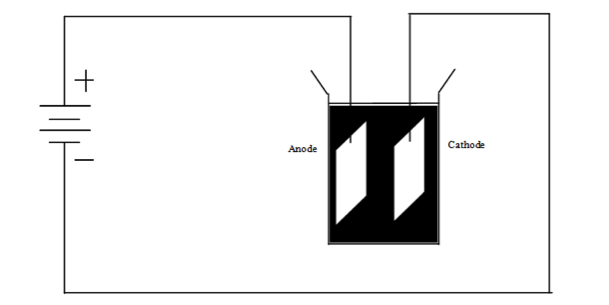
\includegraphics{anodSetup}
\caption{Anodization Setup}
\label{fig_sim}
\end{figure}

Figure 1: Anodization setup

Referring to Fig1, in the simplest case, the current transfer is an ionic transfer where the Ti anode reacts with O2 to create a TiO2 oxide layer. The reaction at the metal-oxide surface can be written as:

Ti + 02 => TiO2 + 4e(equ. 1)

The titanium also reacts with the electrolyte solution to give off hydrogen:

Ti + 2H20 => Ti02 + 4H+Ti02(equ 2)

This hydrogen reacts with the electrons at the cathode to create hydrogen gas and complete the ionic circuit.

4H + 4e => 2H20(equ 3)


This process is very similar to anodizing aluminum. For an explanation of that process visit (---quote Case encyclopedia). 

Since the rate of oxide formation is dependent on the charge transport into the anode during anodization, a current source was selected. A typical anodization process with a current source will see the current and voltage progress as in Fig2
 
Figure 2: Anodization by a Constant Current – quote microminiturization

If a constant current is introduced, the voltage will (ideally) rise linearly with time. This will happen until the DUT reaches the compliance voltage, at which point the current through the DUT will begin to drop off until it reaches the leakage current of the unpackaged capacitor. 


% needed in second column of first page if using \IEEEpubid
%\IEEEpubidadjcol

\subsubsection{Subsubsection Heading Here}
Subsubsection text here.


\appendices
\section{Proof of the First Zonklar Equation}
Appendix one text goes here.

% you can choose not to have a title for an appendix
% if you want by leaving the argument blank
\section{}
Appendix two text goes here.


% use section* for acknowledgement
\section*{Acknowledgment}


The authors would like to thank...


% Can use something like this to put references on a page
% by themselves when using endfloat and the captionsoff option.
\ifCLASSOPTIONcaptionsoff
  \newpage
\fi



% trigger a \newpage just before the given reference
% number - used to balance the columns on the last page
% adjust value as needed - may need to be readjusted if
% the document is modified later
%\IEEEtriggeratref{8}
% The "triggered" command can be changed if desired:
%\IEEEtriggercmd{\enlargethispage{-5in}}

% references section

% can use a bibliography generated by BibTeX as a .bbl file
% BibTeX documentation can be easily obtained at:
% http://www.ctan.org/tex-archive/biblio/bibtex/contrib/doc/
% The IEEEtran BibTeX style support page is at:
% http://www.michaelshell.org/tex/ieeetran/bibtex/
%\bibliographystyle{IEEEtran}
% argument is your BibTeX string definitions and bibliography database(s)
%\bibliography{IEEEabrv,../bib/paper}
%
% <OR> manually copy in the resultant .bbl file
% set second argument of \begin to the number of references
% (used to reserve space for the reference number labels box)
\begin{thebibliography}{1}

\bibitem{IEEEhowto:kopka}
H.~Kopka and P.~W. Daly, \emph{A Guide to \LaTeX}, 3rd~ed.\hskip 1em plus
  0.5em minus 0.4em\relax Harlow, England: Addison-Wesley, 1999.

\end{thebibliography}

% biography section
% 
% If you have an EPS/PDF photo (graphicx package needed) extra braces are
% needed around the contents of the optional argument to biography to prevent
% the LaTeX parser from getting confused when it sees the complicated
% \includegraphics command within an optional argument. (You could create
% your own custom macro containing the \includegraphics command to make things
% simpler here.)
%\begin{biography}[{\includegraphics[width=1in,height=1.25in,clip,keepaspectratio]{mshell}}]{Michael Shell}
% or if you just want to reserve a space for a photo:

\begin{IEEEbiography}{Michael Shell}
Biography text here.
\end{IEEEbiography}

% if you will not have a photo at all:
\begin{IEEEbiographynophoto}{John Doe}
Biography text here.
\end{IEEEbiographynophoto}

% insert where needed to balance the two columns on the last page with
% biographies
%\newpage

\begin{IEEEbiographynophoto}{Jane Doe}
Biography text here.
\end{IEEEbiographynophoto}

% You can push biographies down or up by placing
% a \vfill before or after them. The appropriate
% use of \vfill depends on what kind of text is
% on the last page and whether or not the columns
% are being equalized.

%\vfill

% Can be used to pull up biographies so that the bottom of the last one
% is flush with the other column.
%\enlargethispage{-5in}



% that's all folks
\end{document}


